\chapter{Results}
\label{sec:results}
% again appendix
In this chapter, the results of the experiments are presented. The results for each different problem sets are presented separately. Note that the HPE error detection task can be seen as a classification task, where an error, e.g. an erroneous joint, is considered positive and no error is considered negative. Therefore, a result is considered as a "True Positive", if the ground truth label of a joint is equal to "Error" and the predicted value of that joint is also equal to "Error". Models which suffered from neural collapse are omitted to reduce confusion.

\section{FESDModelv1 Results}
\label{sec:FESDModelv1_results}

After training all four models using FESDModelv1, the results are evaluated. Table \ref{tab:res_v1} shows the results of the testing after 100 epochs of training. The results seem promising with an accuracy in the range of 80 to 90 percent. Additionally, the Cohen's Kappa coefficient shows results in a good range.

\begin{table}
  \caption[Test Results of FESDModelv1]{The test results of FESDModelv1 after 100 epochs of training.}
  \label{tab:res_v1}
  \centering
  \begin{tabular}{p{0.15\linewidth}p{0.15\linewidth}p{0.15\linewidth}p{0.15\linewidth}p{0.15\linewidth}}
    \hline
    {} &  Percentage of positive guesses &  Accuracy &  F1-Score &  Cohen's Kappa Coefficient \\
    Problem Set   &                                 &           &           &                            \\
    \hline
    Full Body  &                          71.667 &     0.842 &     0.642 &                      0.528 \\
    Half Body  &                          64.375 &     0.840 &     0.525 &                      0.622 \\
    Body Parts &                          93.681 &     0.917 &     0.864 &                      0.677 \\
    Joints     &                          69.990 &     0.893 &     0.638 &                      0.773 \\
    \hline
  \end{tabular}
\end{table}

To understand these results the cofusion matrix and ROC curve were calculated. The confusion matrices can be seen in figure \ref{fig:conf_v1} and ROC curves can be seen in figure \ref{fig:roc_v1}. The confusion matrix seems to reflect the results of table \ref{tab:res_v1}. However, the ROC curve shows that the results are as good as they are due to overconfidence and possibly overfitting of the data.

\begin{figure}[ht]
  \centering
  \begin{subfigure}[b]{0.47\linewidth}
      \centering
      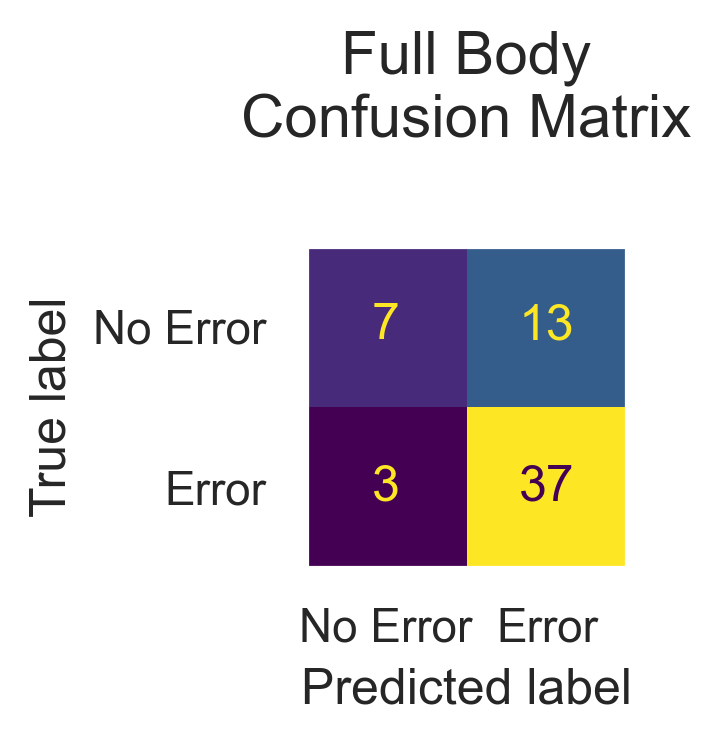
\includegraphics[width=\textwidth]{figures/Results/v1/confusion/full_together.png}
      \caption[]{Full Body Problem Set}
      \label{fig:fb_conf_v1}
  \end{subfigure}
  \hfill
  \begin{subfigure}[b]{0.47\linewidth}
      \centering
      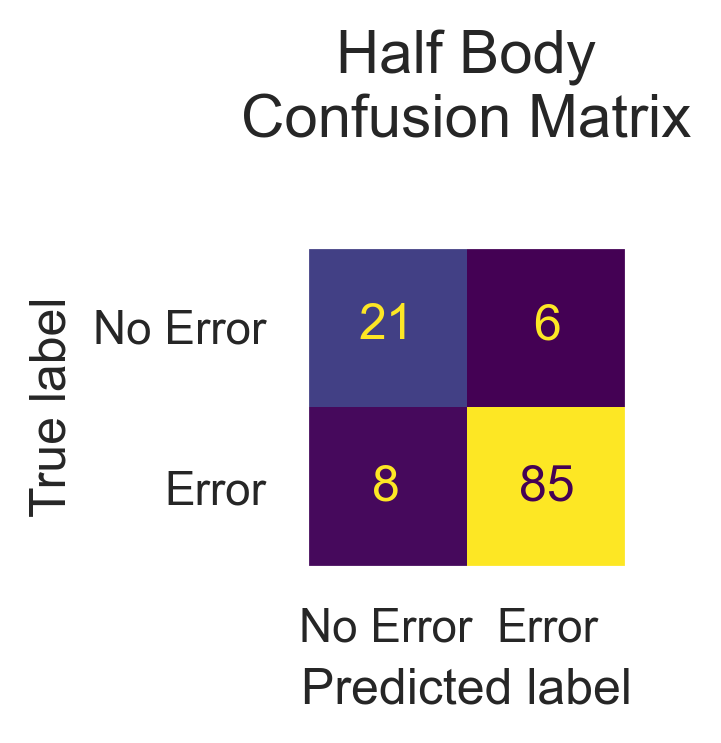
\includegraphics[width=\textwidth]{figures/Results/v1/confusion/half_together.png}
      \caption[]{Half Body Problem Set}
      \label{fig:hb_conf_v1}
  \end{subfigure}
  \hfill
  \begin{subfigure}[b]{0.47\linewidth}
      \centering
      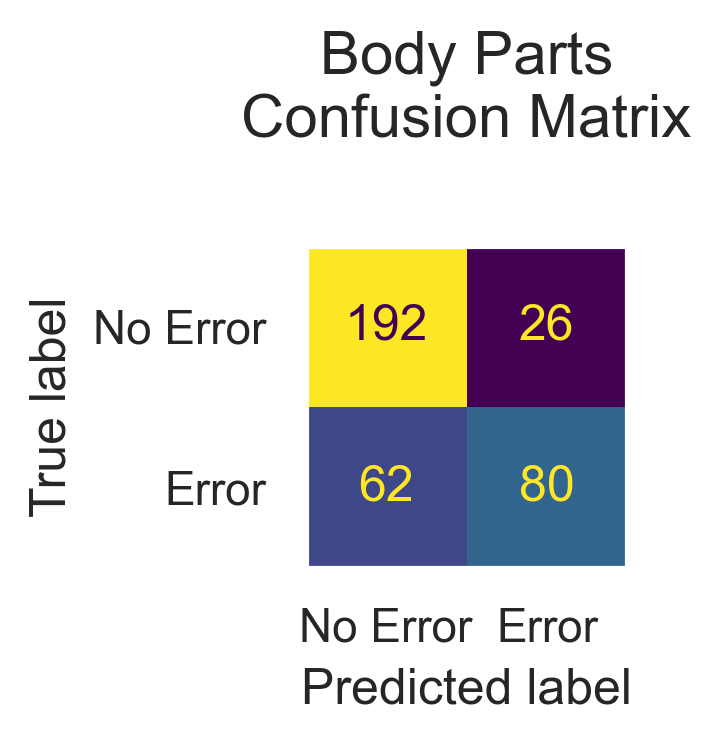
\includegraphics[width=\textwidth]{figures/Results/v1/confusion/body_parts_together.png}
      \caption[]{Body Part Problem Set}
      \label{fig:bp_conf_v1}
  \end{subfigure}
  \hfill
  \begin{subfigure}[b]{0.47\linewidth}
      \centering
      \includegraphics[width=\textwidth]{figures/Results/v1/confusion/joints_together.png}
      \caption[]{Joint Problem Set}
      \label{fig:jt_conf_v1}
  \end{subfigure}
  \caption[Confusion Matrices of FESDModelv1]{The confusion Matrices of FESDModelv1.}
  \label{fig:conf_v1}
\end{figure}

\begin{figure}
  \centering
  \begin{subfigure}[b]{0.47\linewidth}
      \centering
      \includegraphics[width=\textwidth]{figures/Results/v1/fb/roc.png}
      \caption[]{Full Body Problem Set}
      \label{fig:fb_roc_v1}
  \end{subfigure}
  \hfill
  \begin{subfigure}[b]{0.47\linewidth}
      \centering
      \includegraphics[width=\textwidth]{figures/Results/v1/hb/roc.png}
      \caption[]{Half Body Problem Set}
      \label{fig:hb_roc_v1}
  \end{subfigure}
  \hfill
  \begin{subfigure}[b]{0.47\linewidth}
      \centering
      \includegraphics[width=\textwidth]{figures/Results/v1/bp/roc.png}
      \caption[]{Body Part Problem Set}
      \label{fig:bp_roc_v1}
  \end{subfigure}
  \hfill
  \begin{subfigure}[b]{0.47\linewidth}
      \centering
      \includegraphics[width=\textwidth]{figures/Results/v1/jt/roc.png}
      \caption[]{Joint Problem Set}
      \label{fig:jt_roc_v1}
  \end{subfigure}
  \caption[ROC Curves of FESDModelv1]{The ROC curves of FESDModelv1.}
  \label{fig:roc_v1}
\end{figure}

The results for the table and the confusion matrices were summarised over all areas in a problem set, therefore, these seemingly positive values occur. If the areas are considered individually it can be seen that the model is overfitting for each of the areas and mainly predicting a single value. This produces good accuracy since the dataset is unbalanced.
\section{FESDModelv2 Results}

The results of the testing after 50 epochs of training for FESDModelv2 can be seen in table \ref{tab:res_v2}. The numeric values of the accuracy and F1-Score show good results. However, the percentage of positive guesses metric seems to hint at overfitting.

\begin{table}[!htbp]
  \caption[Test Results of FESDModelv1]{The test results of FESDModelv1 after 50 epochs of training.}
  \label{tab:res_v1}
  \begin{tabular}{lrrrrr}
    \hline
    {} &  Percentage of positive guesses &  Accuracy &  F1-Score &  F2-Score &  Cohen's Kappa Coefficient \\
    Problem Set   &                                 &           &           &           &                            \\
    \hline
    Full Body  &                          50.417 &     0.688 &     0.458 &     0.673 &                      0.397 \\
    Half Body  &                          55.833 &     0.767 &     0.446 &     0.789 &                      0.554 \\
    Body Parts &                          79.028 &     0.779 &     0.722 &     0.842 &                      0.257 \\
    Joints     &                          70.000 &     0.892 &     0.638 &     0.918 &                      0.773 \\
    \hline
  \end{tabular}
\end{table}

The results shown in table \ref{tab:res_v2} are reflected in the confusion matrices seen in figure \ref{fig:conf_v2}. The half-body and body parts problem set only guess positive results, hence the Percentage of positive guesses. The Cohen's Kappa Coefficient is 0 if $tp \cdot tn = fn \cdot fp$. This is the case if only one class is guessed, which is the case if all guesses are positive.

\begin{figure}[htbp]
  \centering
  \begin{subfigure}[b]{0.4\linewidth}
      \centering
      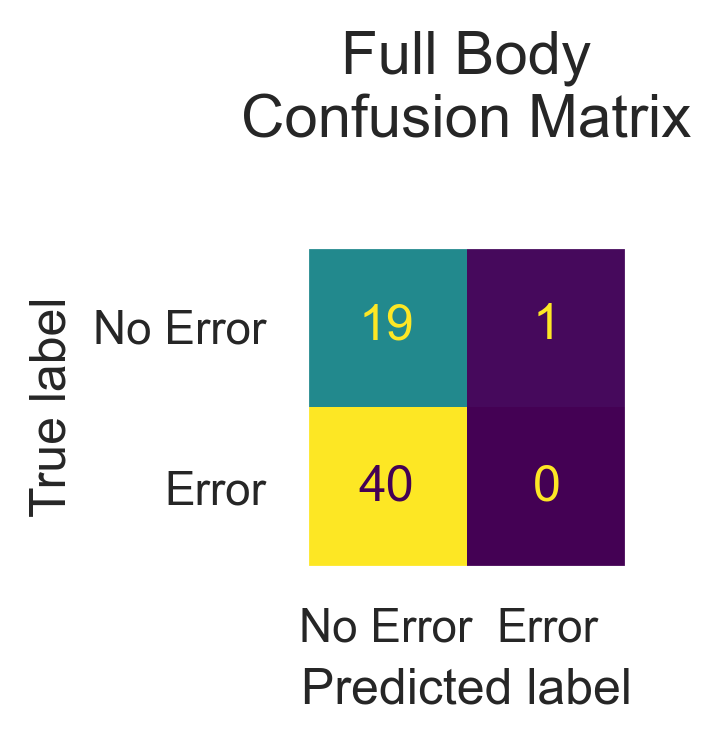
\includegraphics[width=\textwidth]{figures/Results/v2/confusion/full_together.png}
      \caption[]{Full Body Problem Set}
      \label{fig:fb_conf}
  \end{subfigure}
  \hfill
  \begin{subfigure}[b]{0.4\linewidth}
      \centering
      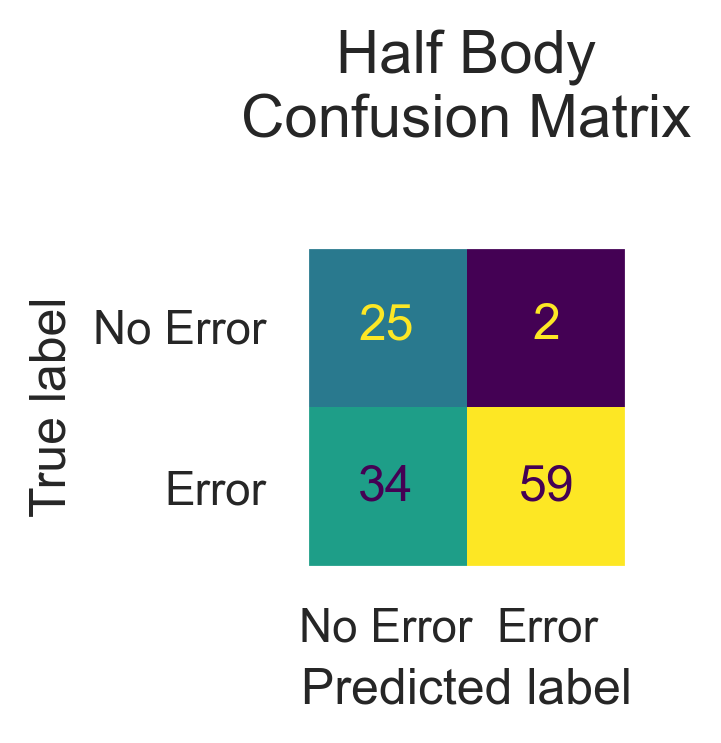
\includegraphics[width=\textwidth]{figures/Results/v2/confusion/half_together.png}
      \caption{Half Body Problem Set}
      \label{fig:hb_conf}
  \end{subfigure}
  \hfill
  \begin{subfigure}[b]{0.4\linewidth}
      \centering
      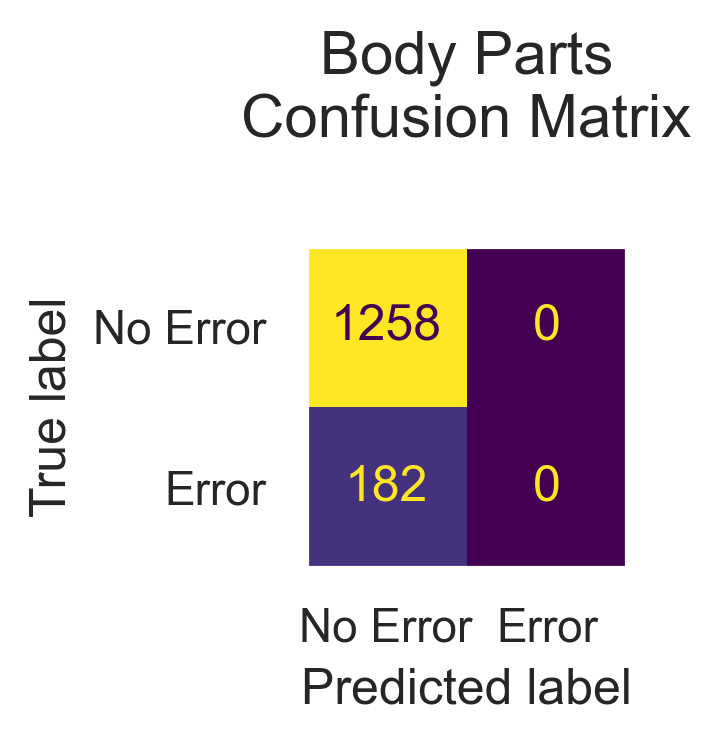
\includegraphics[width=\textwidth]{figures/Results/v2/confusion/body_parts_together.png}
      \caption{Body Part Problem Set}
      \label{fig:bp_conf}
  \end{subfigure}
  \hfill
  \begin{subfigure}[b]{0.4\linewidth}
      \centering
      \includegraphics[width=\textwidth]{figures/Results/v2/confusion/joints_together.png}
      \caption{Joint Problem Set}
      \label{fig:jt_conf}
  \end{subfigure}
  \caption[Confusion Matrices of FESDModelv2]{The confusion Matrices of FESDModelv2.}
  \label{fig:conf_v2}
\end{figure}

The ROC-curves shown in figure \ref{fig:roc_v2}, show the different true positive and false positive rates for each of the areas in each problem set.

\begin{figure}[htbp]
  \centering
  \begin{subfigure}[b]{0.4\linewidth}
      \centering
      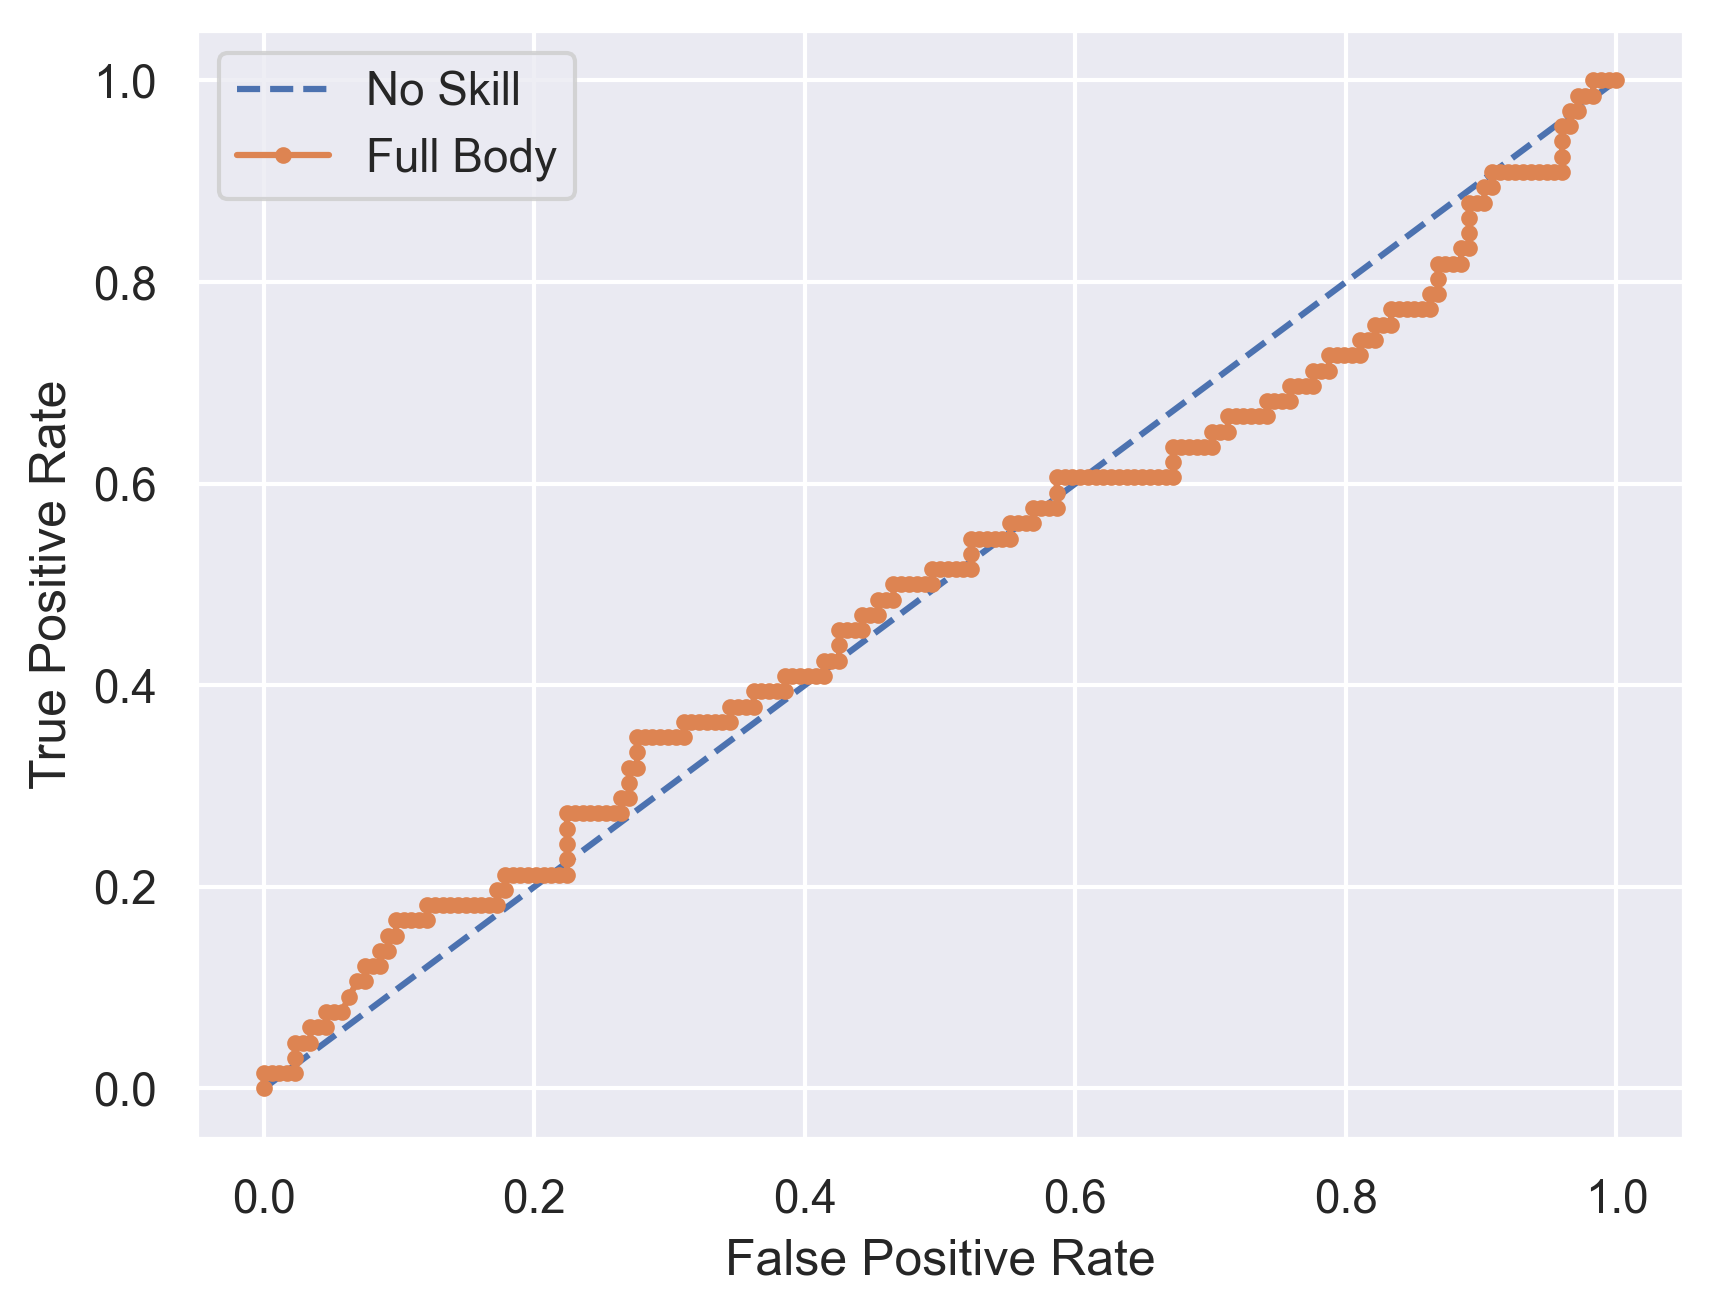
\includegraphics[width=\textwidth]{figures/Results/v2/roc/fb.png}
      \caption[]{Full Body Problem Set}
      \label{fig:fb_roc_v2}
  \end{subfigure}
  \hfill
  \begin{subfigure}[b]{0.4\linewidth}
      \centering
      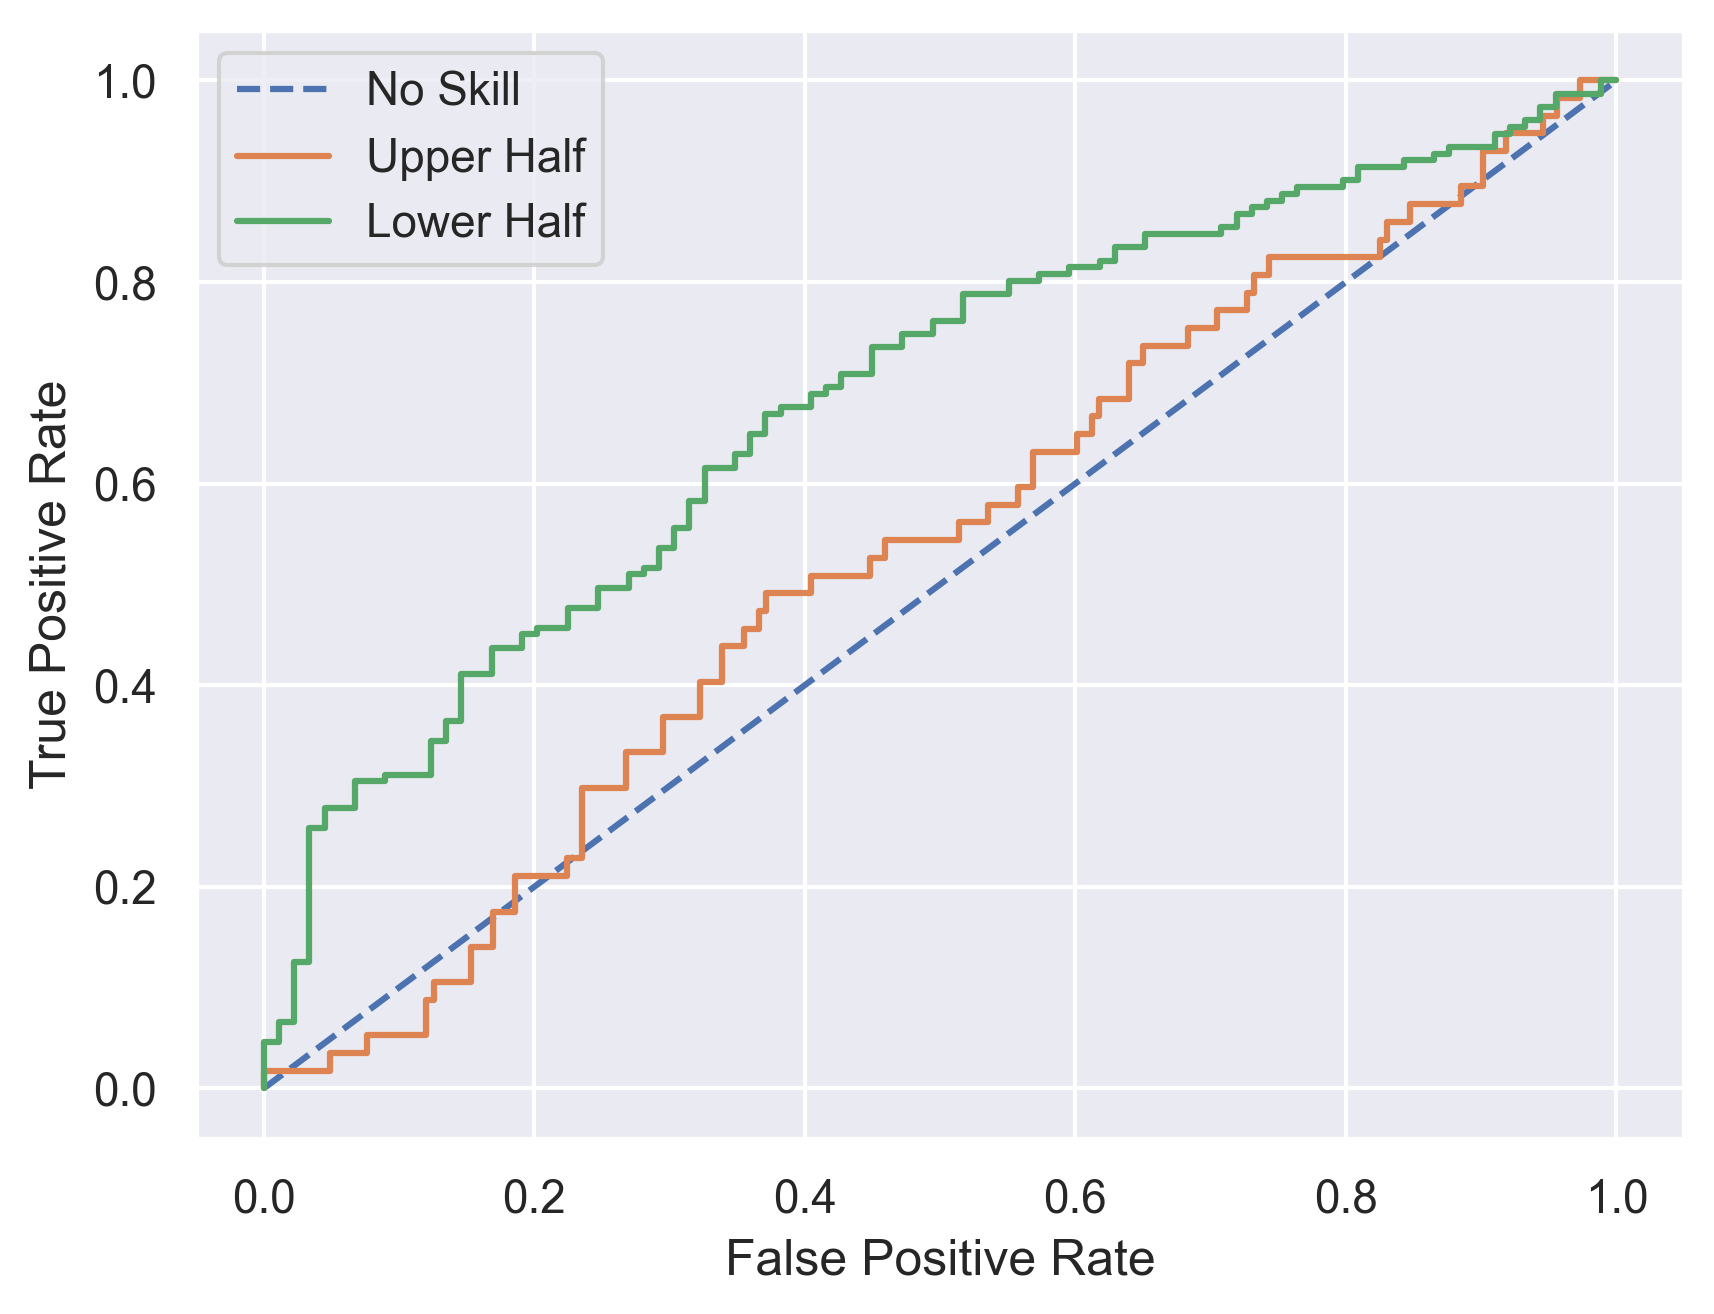
\includegraphics[width=\textwidth]{figures/Results/v2/roc/hb.png}
      \caption[]{Half Body Problem Set}
      \label{fig:hb_roc_v2}
  \end{subfigure}
  \hfill
  \begin{subfigure}[b]{0.4\linewidth}
      \centering
      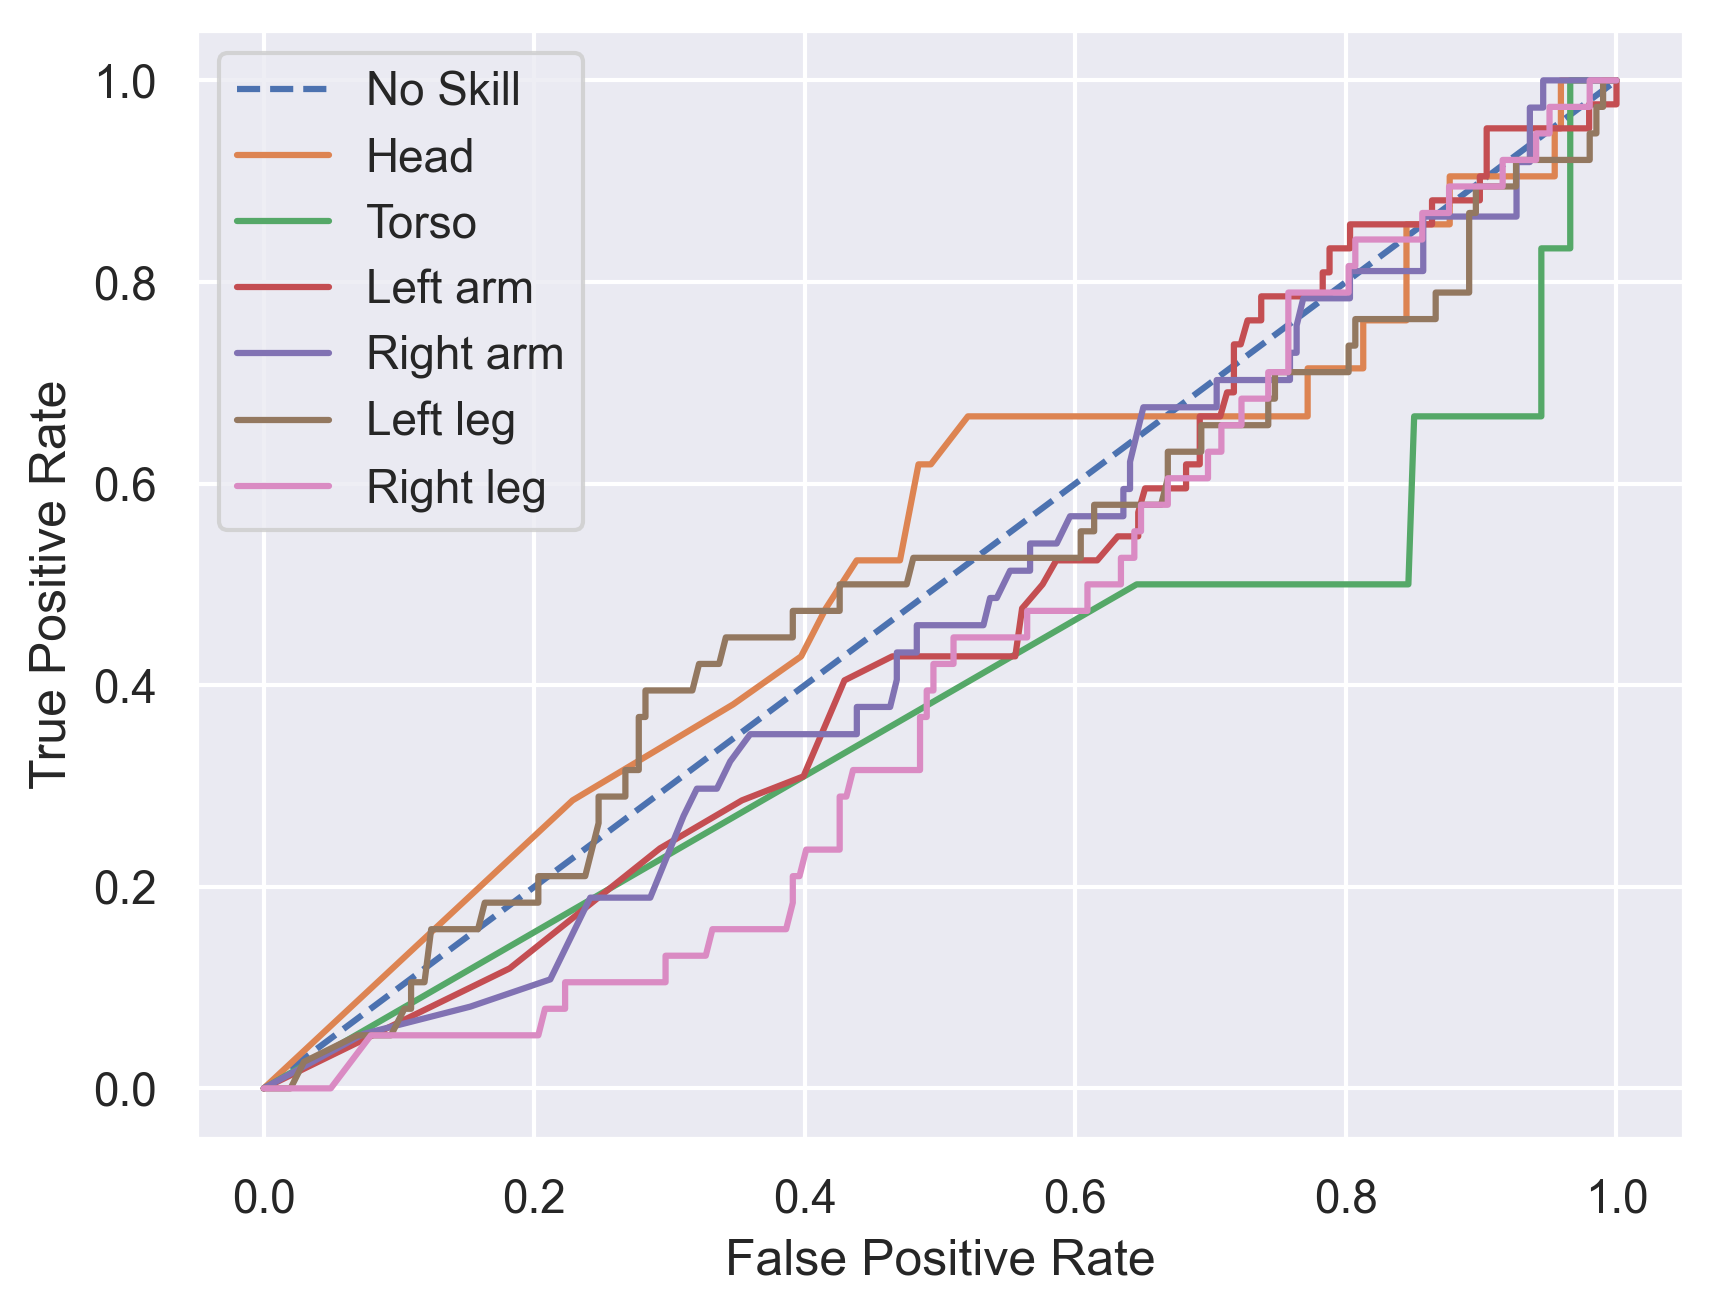
\includegraphics[width=\textwidth]{figures/Results/v2/roc/bp.png}
      \caption[]{Body Part Problem Set}
      \label{fig:bp_roc_v2}
  \end{subfigure}
  \hfill
  \begin{subfigure}[b]{0.4\linewidth}
      \centering
      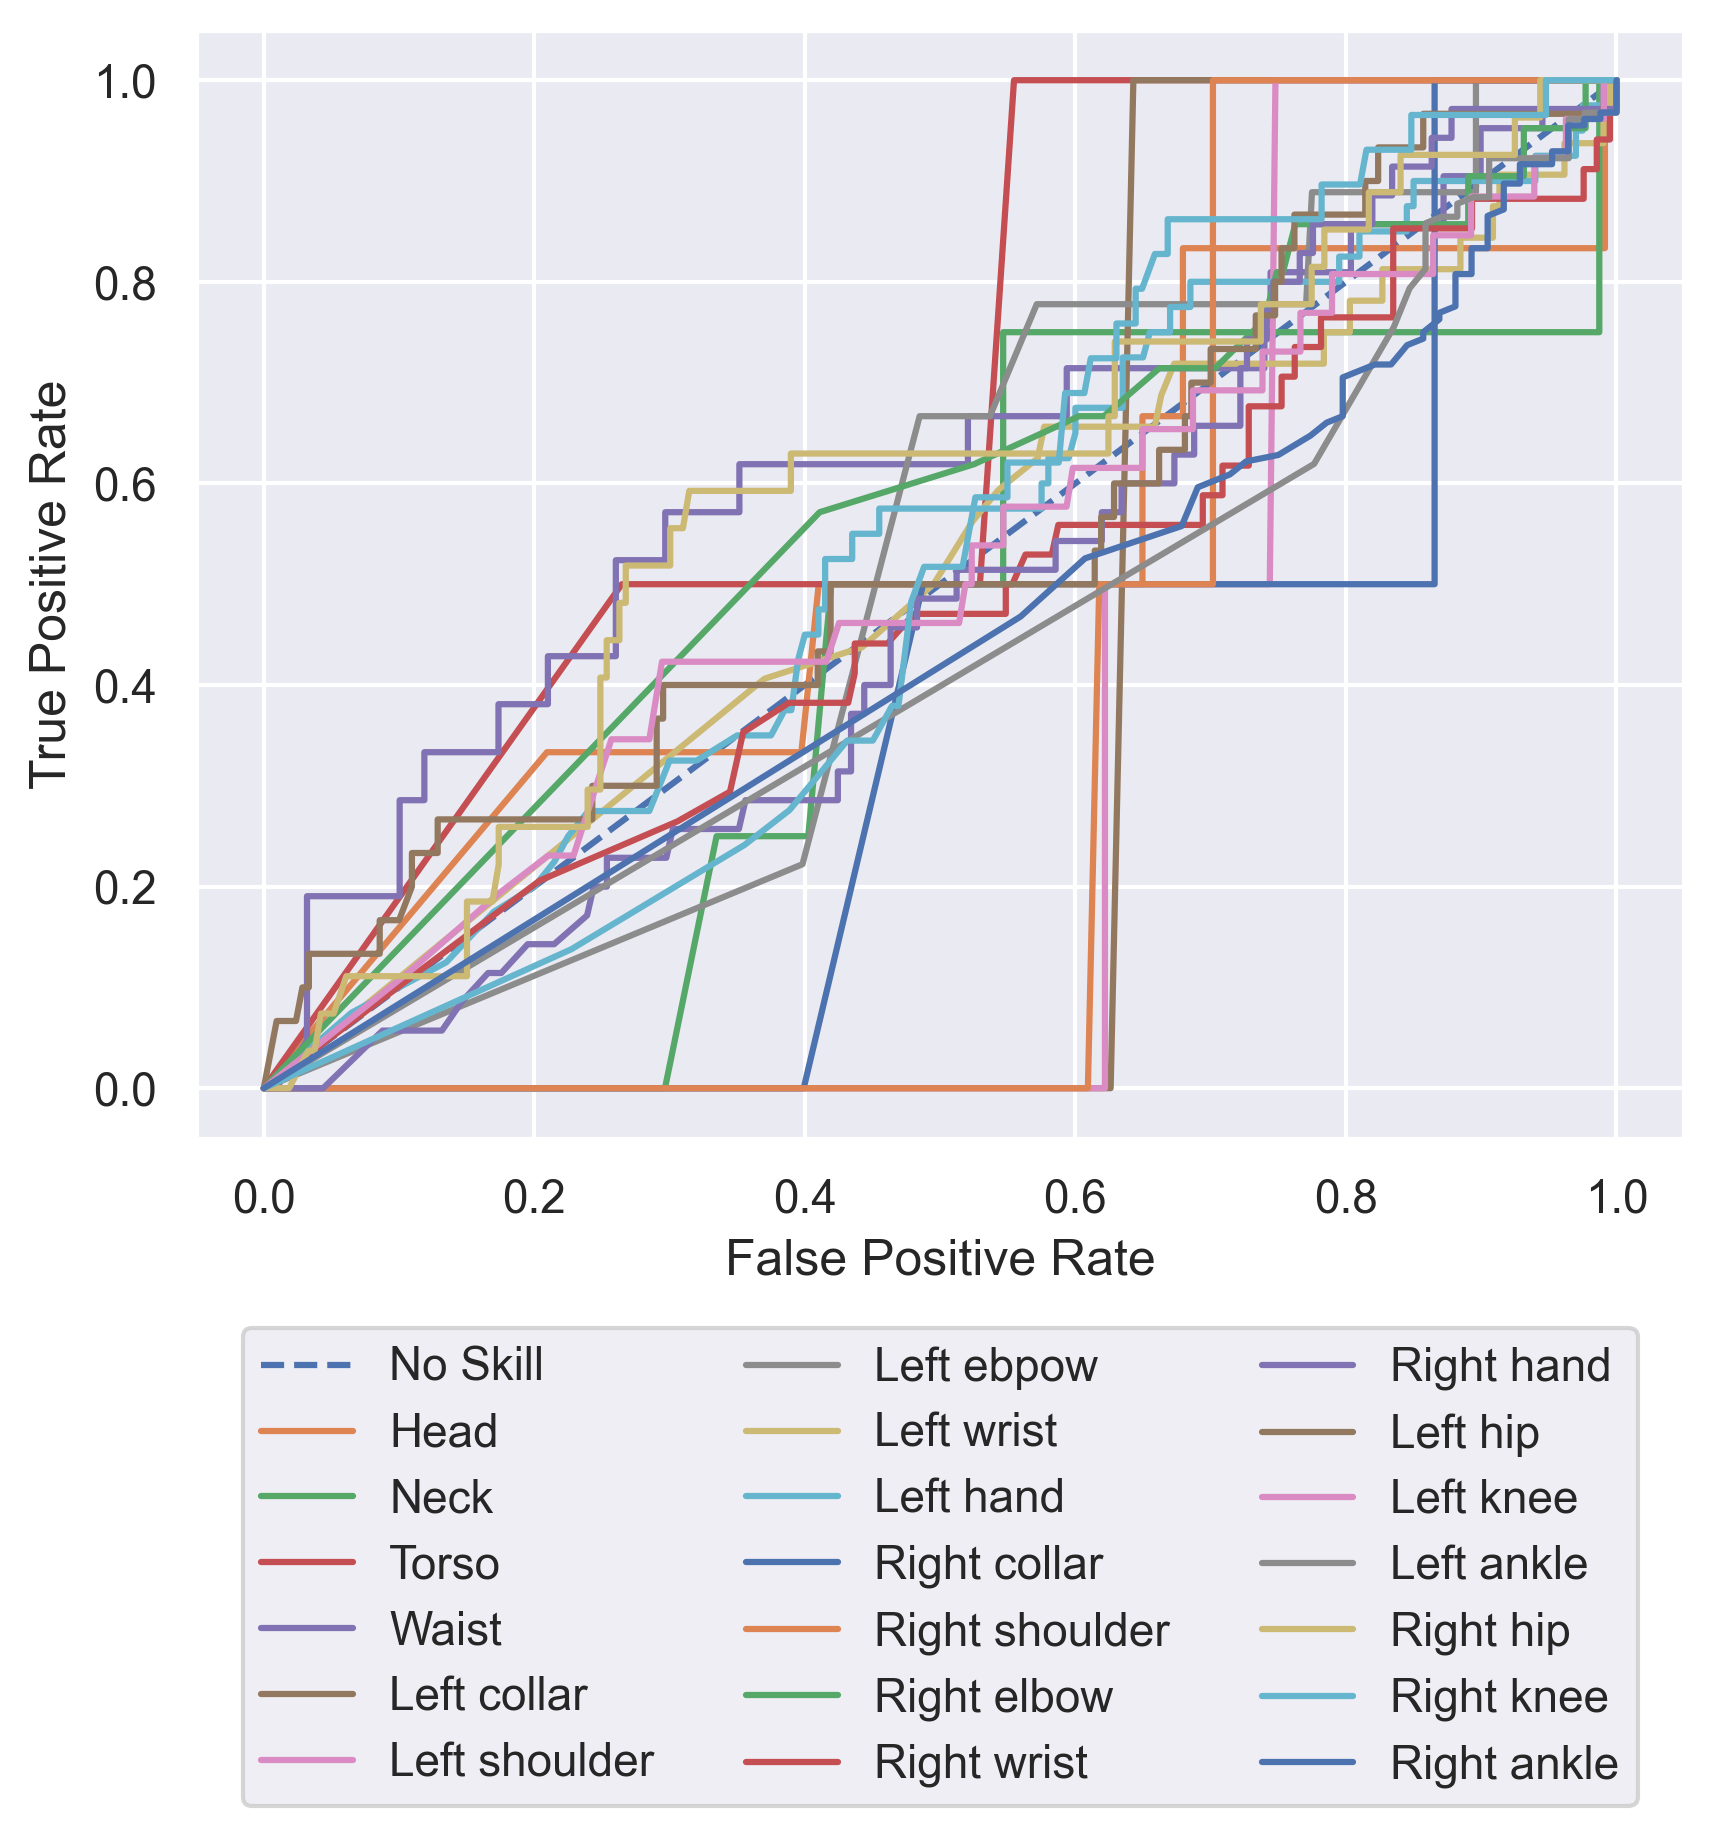
\includegraphics[width=\textwidth]{figures/Results/v2/roc/jt.png}
      \caption[]{Joint Problem Set}
      \label{fig:jt_roc_v2}
  \end{subfigure}
  \caption[ROC Curves of FESDModelv2]{The ROC curves of FESDModelv2.}
  \label{fig:roc_v2}
\end{figure}

The Joint model seems like it is getting good results when considering all joints together. However, when considering the confusion matrix for each of the joints, as can be seen in figure \ref{fig:conf_v2_jts}, the show that while in total not a single error label is guessed all the time for all joints together, each joint does not have varying error labels and is therefore not a good model. 

\begin{figure}[htbp]
  \centering
  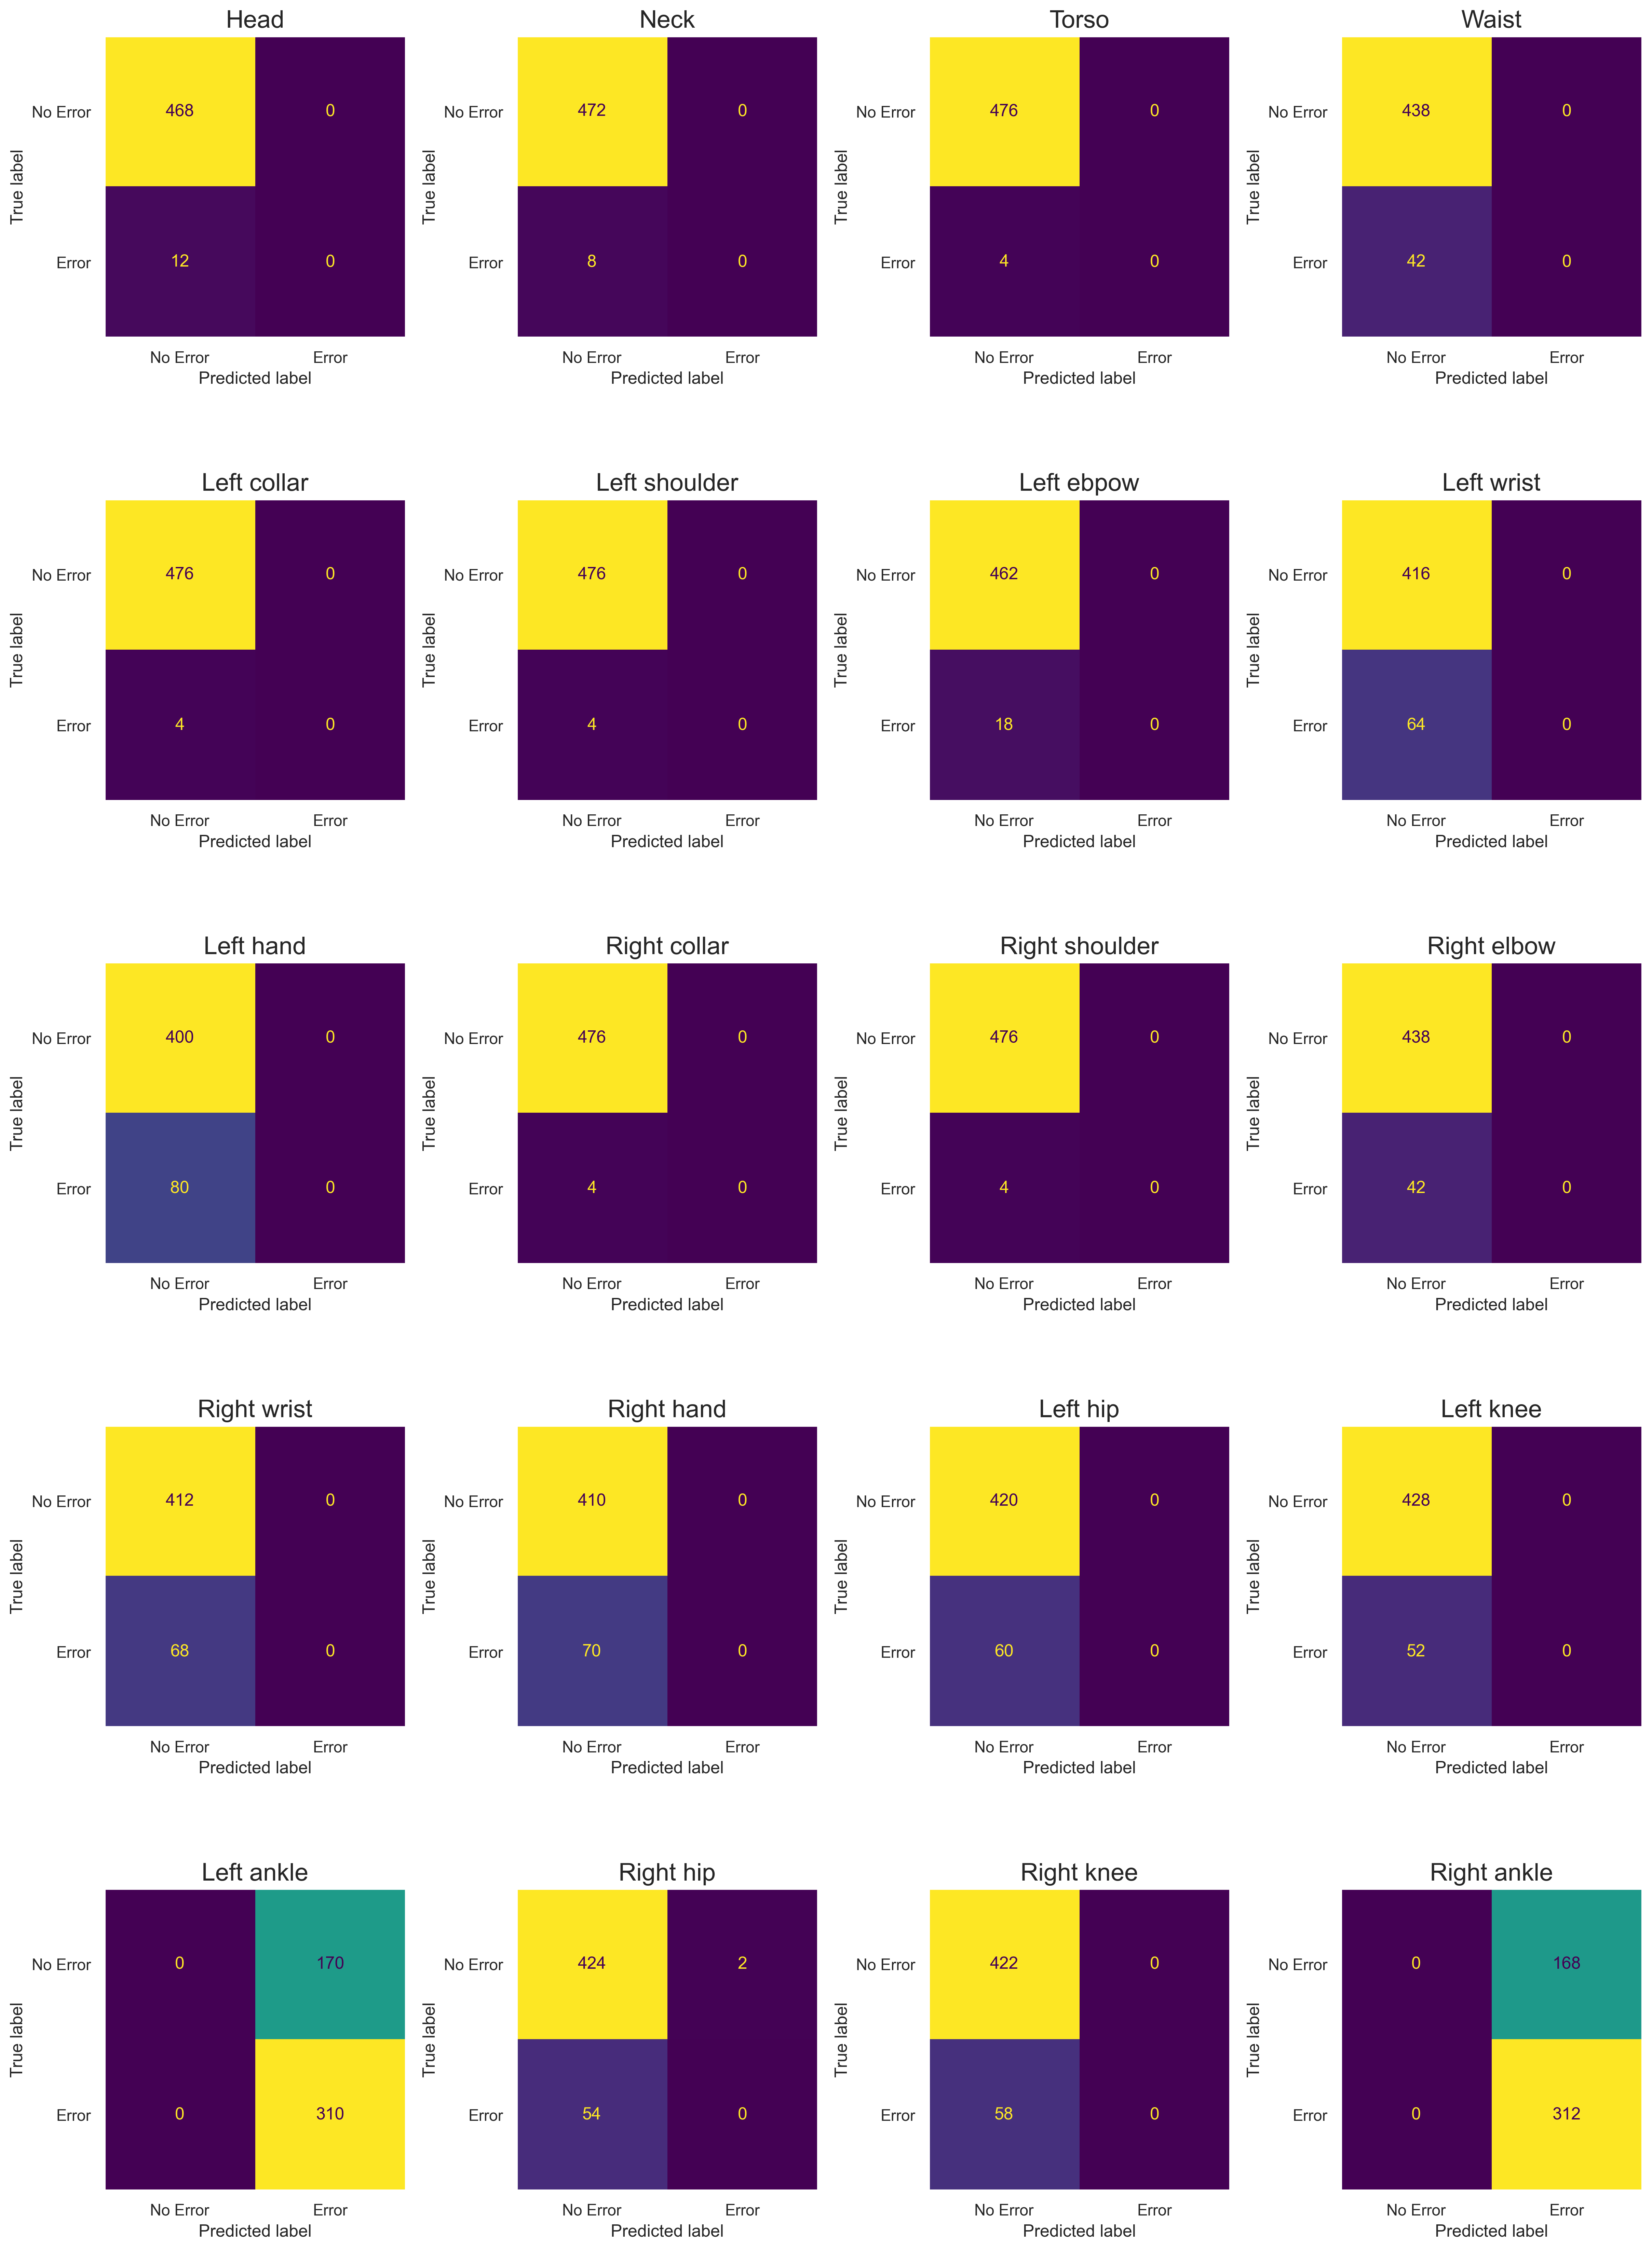
\includegraphics[width=.8\linewidth]{figures/Results/v2/confusion/joints_joint.png}
  \caption[Confusion matrix of FESDModelv2 for each Joint]{The confusion matrix of each joint for FESDModelv2 for the joint problem set.}
  \label{fig:conf_v2_jts}
\end{figure}

Similar to FESDModelv1, the Half Body problem set is getting very good results which do not indicate overfitting. In figure \ref{fig:conf_v2_hb_ul} the confusion matrices can be seen for the upper and lower body. It can be seen that the detection of the lower body is more successful than the detection of the upper body. It is important to consider, that the upper body has far more stable joints and more joints in general. This discrepancy might be the reason for the diverging accuracy of the upper and lower body.

\begin{figure}[htbp]
  \centering
  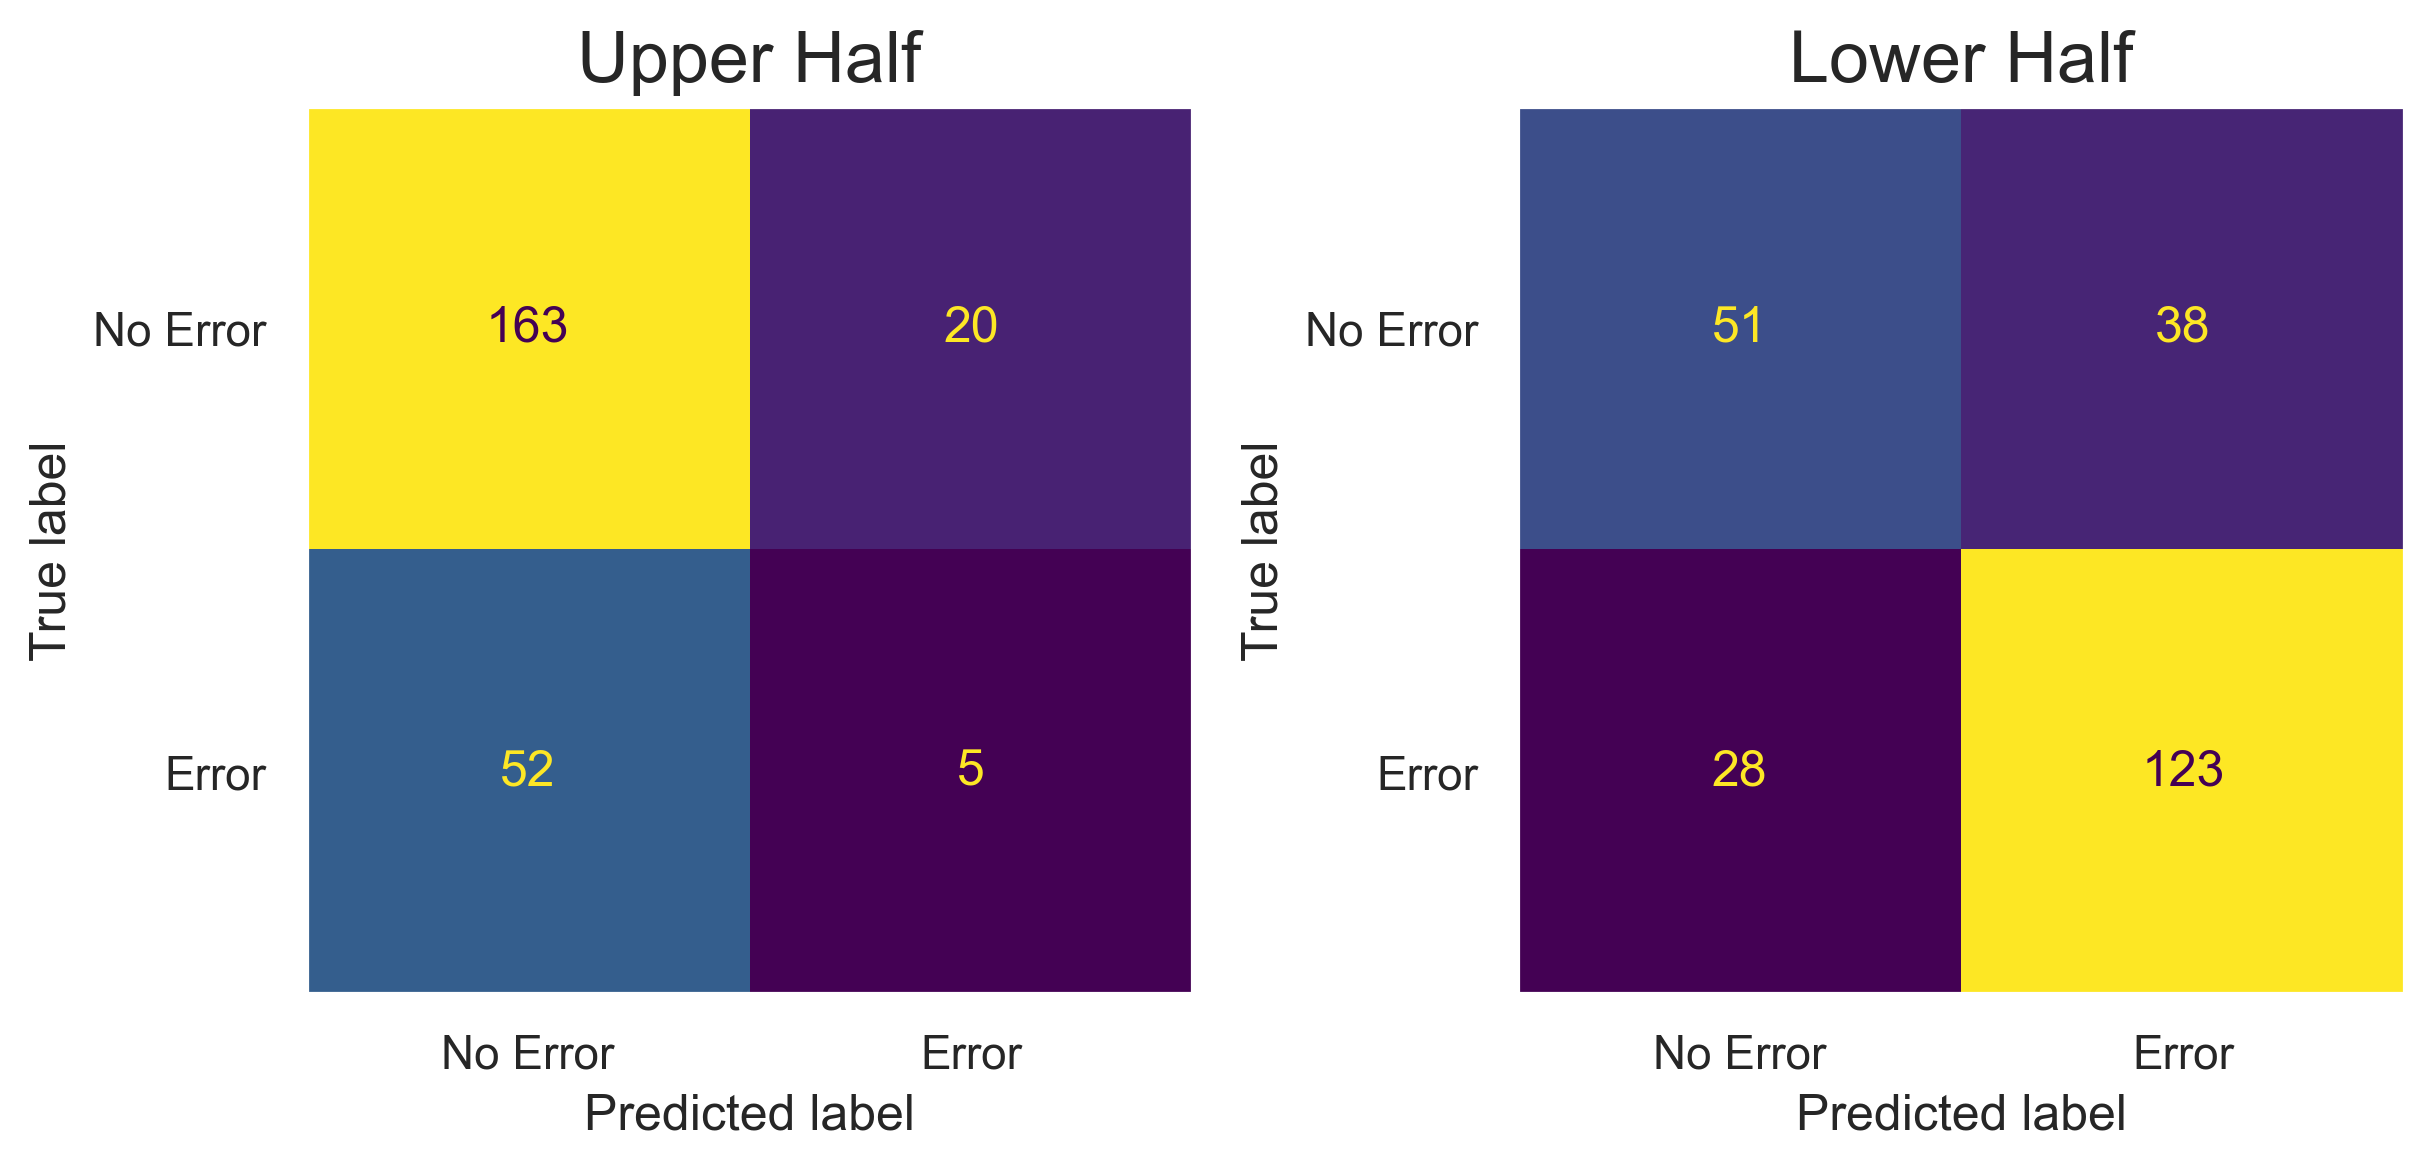
\includegraphics[width=.8\linewidth]{figures/Results/v2/confusion/body_halves_half.png}
  \caption[Confusion matrix of FESDModelv2 for each Body Half]{The confusion matrix of the upper and lower body for FESDModelv2 for the body half problem set.}
  \label{fig:conf_v2_hb_ul}
\end{figure}

\FloatBarrier
